\documentclass[presentation, shownotes]{beamer}
\setbeamercovered{transparent}

\mode<presentation> {
    \usetheme{Frankfurt}
    \usecolortheme{whale}
    %\setbeamertemplate{footline} % remove the footer line
    %\setbeamertemplate{footline}[page number] % replace the footer line
    \setbeamertemplate{navigation symbols}{} % remove nav symbols
}

\usepackage[T1]{fontenc}
\usepackage[ngerman]{babel}
\usepackage[utf8]{inputenc}
\usepackage{graphicx}
\usepackage{booktabs}
\usepackage{listings}
\usepackage[
    backend=biber,
    style=authoryear,
    sorting=nyt,
    citestyle=authoryear]{biblatex}
\addbibresource{Literatur.bib}
\usepackage{csquotes}
\usepackage{relsize}

\graphicspath {{figures/}}

%c from texinfo.tex
\def\ifmonospace{\ifdim\fontdimen3\font=0pt }

% prettier C++ formatting
\def\C++{%
\ifmonospace%
    C++%
\else%
    C\kern-.1667em\raise.30ex\hbox{\smaller{++}}%
\fi%
\spacefactor1000 }

%------------------------------------------------
%    TITLE PAGE
%------------------------------------------------

\title[Haskell vs. C++]{Vergleich paralleler Datenverarbeitung in Haskell und C++ anhand eines MapReduce Szenarios}

\author{Hans Christian Rudolph}
\institute[HfTL] {
    Hochschule für Telekommunikation Leipzig\\
    \medskip
    \textit{hans-christian.rudolph@hft-leipzig.de}\\
    \textit{@hcrudolph}
}
\date{12. Oktober 2016}

\begin{document}

\begin{frame}
    \titlepage
\end{frame}

\begin{frame}
    \frametitle{Gliederung}
    \tableofcontents
\end{frame}

%------------------------------------------------
%    PRESENTATION SLIDES
%-----------------------------------------------

%------------------------------------------------
\section{Einleitung}
\setcounter{subsection}{1}
%------------------------------------------------

\begin{frame}[plain]{}
    \footnotesize{
    Warum sollten sich Programmierende mit den Konzepten funktionaler Sprachen auseinandersetzen? Schließlich existiert eine Vielzahl von Alternativen, die einfacher zu erlernen sind, eine deutlich größere Ver- breitung genießen und mehr Community-Unterstützung erfahren.
    Die Antwort ist denkbar einfach: weil die grundverschiedenen Herangehensweisen dieses Paradigmas den Horizont erweitern und neue, effiziente Lösungswege zu bestehenden Problemen offenbaren können.
    Wer sich mit einer dieser Programmiersprachen befasst hat, wird das Gelernte auch auf andere Bereiche transferieren und so zu expressivem, sicherem und leicht wartbarem Quellcode beitragen.
    Diese Erkenntnis ist auch an etablierten Sprachen, wie \C++, C\# und Java, nicht spurlos vorbeigegangen.
    Obgleich sich ein rein funktionales Vorgehen nicht für jeden Anwendungsfall eignet, ist hier der deutliche Trend zu beobachten, stetig mehr funktionale Komponenten zu integrieren -- ein erster Schritt in Richtung maximal modularer, zukunftsfähiger Softwareprojekte.
}
\end{frame}

%------------------------------------------------

\begin{frame}
\frametitle{Funktional vs. Imperativ}
\begin{columns}[c] % The "c" option specifies centered vertical alignment while the "t" option is used for top vertical alignment
\column{.5\textwidth} % Left column and width
    \textbf{Haskell}
    \begin{itemize}
    \item Rein funktional
    \item Stark abstrahiert
    \item Referenzielle Transparenz
    \end{itemize}

\column{.5\textwidth} % Right column and width
    \textbf{\C++}
    \begin{itemize}
    \item Multiple Paradigmen
    \item (Wenn nötig) hardwarenah
    \item Zero-Cost Abstractions
    \end{itemize}
\end{columns}
\end{frame}

%------------------------------------------------

\begin{frame}[plain]{}
\begin{figure}
\centering

\includegraphics[height=.7\textheight]{parallel}
\end{figure}
\end{frame}

%------------------------------------------------

\begin{frame}
    \centering
    \citeauthor{marlow2009runtime} (\citeyear{marlow2009runtime}, S.1) stellen fest:\\ \bigskip
    \Large{
        ,,Plenty of papers describe promising ideas,\\ but vastly fewer describe real implementations [\dots]''.
    }
\end{frame}

%------------------------------------------------

\begin{frame}[plain]{}
\begin{figure}
\centering

\includegraphics[height=.7\textheight]{sad}
\end{figure}
\end{frame}

%------------------------------------------------

\begin{frame}
\frametitle{Begriffserklärung}

\pause

\onslide<2->{
\begin{block}{Nebenläufigkeit}
    beschreibt die unabhängige Ausführung von Berechnungen. Dies kann sowohl auf paralleler Hardware (mehrere CPUs) als auch auf sequenzieller geschehen.
    Es ist somit nicht ausgeschlossen, dass auch nebenläufige Aufgaben von paralleler Hardware profitieren.
    Das Resultat ist nicht-deterministisch.
    Bsp.: Webserver
\end{block}
}

\onslide<3->{
\begin{block}{Parallelität}
    beschreibt die \textit{gleichzeitige}, unabhängige Ausführung von Berechnungen auf paralleler Hardware.
    Das Resultat ist stets deterministisch.
    Bsp.: Grafikkarte
\end{block}
}

\end{frame}

%------------------------------------------------

\begin{frame}
\frametitle{Szenario}
\begin{itemize}
\setlength\itemsep{1em}
\item Aggregationsfunktion
\item Lokal gespeicherte Textdateien
\item Schlüsselfelder
% \begin{itemize}
%     \item[$-$] \texttt{AggregationsDatum}
%     \item[$-$] \texttt{Eventklasse}
%     \item[$-$] \texttt{Eventsource}
%     \item[$-$] \texttt{Plattform}
%     \item[$-$] \texttt{Tarifzone}
% \end{itemize}
\item Aggregationsfelder \texttt{Dauer} und \texttt{Volumen}
% \begin{itemize}
%     \item[$-$]
%     \item[$-$] \texttt{Volumen}
% \end{itemize}
\item Summiere die Aggregationsfelder für jeden distinkten Schlüssel
\end{itemize}
\end{frame}

%------------------------------------------------

% \begin{frame}
% \frametitle{Multiple Columns}
% \begin{columns}[c] % The "c" option specifies centered vertical alignment while the "t" option is used for top vertical alignment

% \column{.45\textwidth} % Left column and width
% \textbf{Heading}
% \begin{enumerate}
% \item Statement
% \item Explanation
% \item Example
% \end{enumerate}

% \column{.5\textwidth} % Right column and width
% Lorem ipsum dolor sit amet, consectetur adipiscing elit. Integer lectus nisl, ultricies in feugiat rutrum, porttitor sit amet augue. Aliquam ut tortor mauris. Sed volutpat ante purus, quis accumsan dolor.

% \end{columns}
% \end{frame}

%------------------------------------------------
\section[MapReduce]{Das MapReduce Programmiermodell}

\begin{frame}
\tableofcontents[currentsection]
\end{frame}
%------------------------------------------------

\setcounter{subsection}{1}

\begin{frame}
\frametitle{MapReduce}
    \begin{itemize}
        \item Vorgestellt von den Googlern \citeauthor{DBLP:conf/osdi/DeanG04} (\citeyear{DBLP:conf/osdi/DeanG04})
        \item Ziel: Verarbeitung großer Datenmengen auf Clustern handelsüblicher Hardware
        \item Google Framework realisiert Datenverteilung, -sicherung und Fehlerbehandlung während der Übertragung
        \item Auch auf einzelnen Mehrkernrechnern anwendbar\\
        (vgl. \cite{ranger2007evaluating}, \cite{talbot2011phoenix})
        \item Grundlegendes Programmiermodell eignet sich jedoch für eine Vielzahl von Problemen
    \end{itemize}
\end{frame}

%------------------------------------------------

\begin{frame}[fragile]
\frametitle{Map Funktional}
    \begin{block}{Definition}
        Das Funktional Map wendet eine gegebene Funktion \texttt{f} auf sämtliche Elemente einer Sequenz an. Das Resultat ist die Sequenz der einzelnen Funktionswerte.
    \end{block}

    \begin{block}{Beispiele}
    \begin{lstlisting}[language=haskell]
    map (*2) [1,2,3]     = [2,4,6]
    map toUpper "foobar" = "FOOBAR"
    \end{lstlisting}
    \end{block}
\end{frame}

%------------------------------------------------

\begin{frame}[fragile]
\frametitle{Reduce/Fold Funktional}
    \begin{block}{Definition}
        Das Funktional Reduce/Fold wendet eine binäre Funktion auf jedes Element einer Sequenz an.
    \end{block}

    \begin{block}{Beispiel}
    \begin{lstlisting}[language=haskell]
    foldl (+) 0 [1,2,3] = 6

    -- foldl (+) 0             [1,2,3] = ...
    -- foldl (+) (0+1)         [2,3]   = ...
    -- foldl (+) ((0+1)+2)     [3]     = ...
    -- foldl (+) (((0+1)+2)+3) [1,2,3] = 6
    \end{lstlisting}
    \end{block}
\end{frame}

%------------------------------------------------

\begin{frame}
\frametitle{Logische Struktur}
\begin{figure}
\centering
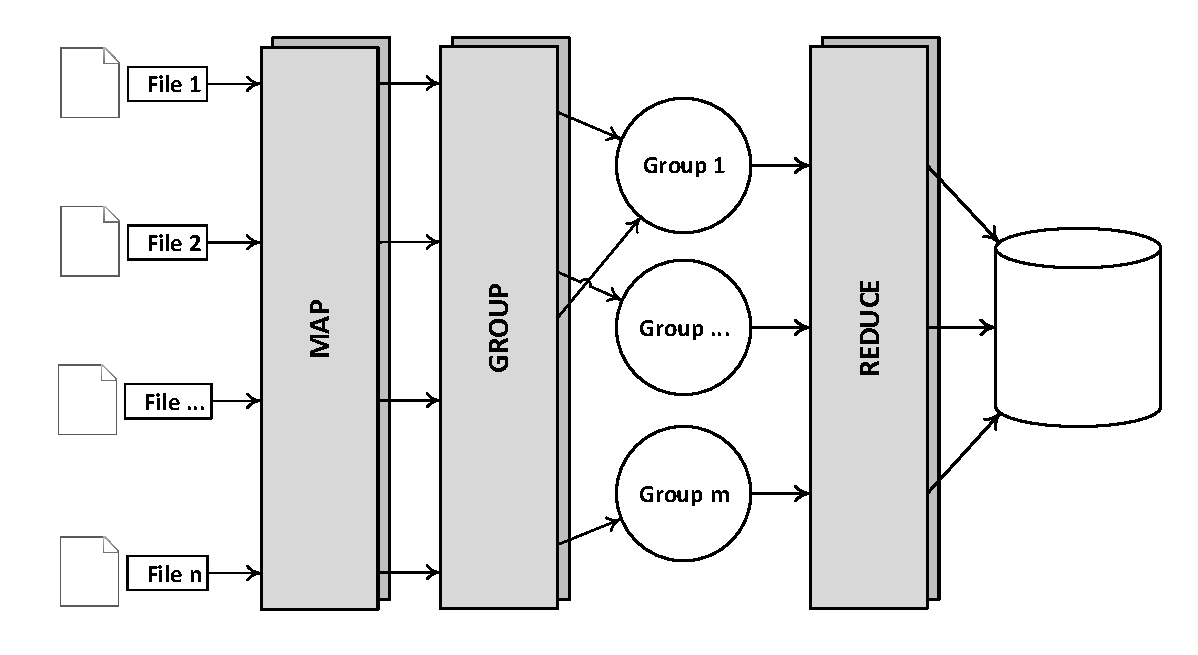
\includegraphics[height=.7\textheight]{mapred.pdf}
\end{figure}
\end{frame}

%------------------------------------------------

% \begin{frame}
% \frametitle{Table}
% \begin{table}
% \begin{tabular}{l l l}
% \toprule
% \textbf{Treatments} & \textbf{Response 1} & \textbf{Response 2}\\
% \midrule
% Treatment 1 & 0.0003262 & 0.562 \\
% Treatment 2 & 0.0015681 & 0.910 \\
% Treatment 3 & 0.0009271 & 0.296 \\
% \bottomrule
% \end{tabular}
% \caption{Table caption}
% \end{table}
% \end{frame}

%------------------------------------------------

% \begin{frame}
% \frametitle{Theorem}
% \begin{theorem}[Mass--energy equivalence]
% $E = mc^2$
% \end{theorem}
% \end{frame}

%------------------------------------------------

% \begin{frame}[fragile] % Need to use the fragile option when verbatim is used in the slide
% \frametitle{Verbatim}
% \begin{example}[Theorem Slide Code]
% \begin{verbatim}
% \begin{frame}
% \frametitle{Theorem}
% \begin{theorem}[Mass--energy equivalence]
% $E = mc^2$
% \end{theorem}
% \end{frame}\end{verbatim}
% \end{example}
% \end{frame}

%------------------------------------------------

% \begin{frame}
% \frametitle{Figure}
% \begin{figure}
% 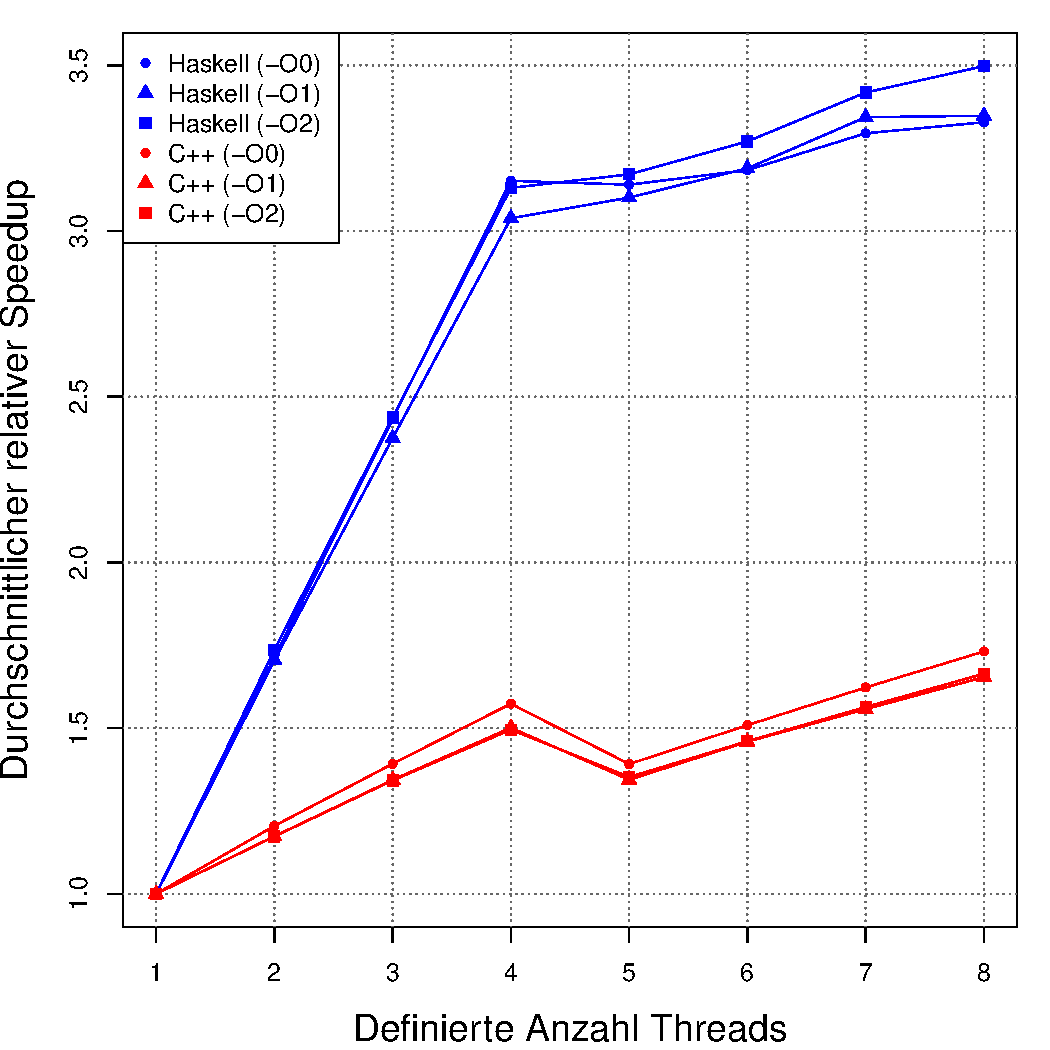
\includegraphics[height=.8\textheight]{speedup_desktop.pdf}
% \end{figure}
% \end{frame}

%------------------------------------------------

% \begin{frame}[fragile] % Need to use the fragile option when verbatim is used in the slide
% \frametitle{Citation}
% An example of the \verb|\cite| command to cite within the presentation:\\~

% This statement requires citation \cite{p1}.
% \end{frame}

%------------------------------------------------
\section{Parallelrechner}

\begin{frame}
\tableofcontents[currentsection]
\setcounter{subsection}{1}
\end{frame}
%------------------------------------------------

\begin{frame}
\frametitle{Flynnsche Klassifizierung}
    \citeauthor{flynn1966very} (\citeyear{flynn1966very}) unterteilt Rechner nach ihrer Prozessoranzahl und den von ihnen gesteuerten Kontroll- und Datenflüssen in vier Kategorien:
    \begin{itemize}
    \setlength\itemsep{1em}
    \item Single Instruction Stream--Single Data Stream (SISD)
    \item Single Instruction Stream--Multiple Data Stream (SIMD)
    \item Multiple Instruction Stream--Single Data Stream (MISD)
    \item Multiple Instruction Stream--Multiple Data Stream (MIMD)
    \end{itemize}
\end{frame}

% \begin{frame}
% \frametitle{Datenparallelismus}
%     \begin{block}{Definition}
%     Die gleichzeitige Anwendung der selben Funktion auf eine Menge von Daten wird auch Datenparallelismus genannt.
%     \end{block}
% \end{frame}

\begin{frame}
\frametitle{Speicheraufbau}
\onslide<2->{
    \begin{block}{Zusammenhängender Speicher}
    Als Multiprozessoren, bzw. \textit{Shared Memory Machines (SMMs)}, werden Rechner bezeichnet, deren CPUs einen physikalisch gemeinsamen Speicher mit zusammenhängendem Adressraum besitzen.
    Die darin enthaltenen Daten stehen allen Prozessoren direkt zur Verfügung und können zwischen ihnen geteilt werden.
    (Vgl. \cite{rauber2012parallele}, S.20ff)
    \end{block}
}
\onslide<3->{
    \begin{block}{Verteilter Speicher}
    \textit{Distributed Memory Machines (DMMs)}, auch Multicomputer genannt, arbeiten mit einem physikalisch separierten Speicher, welcher dem jeweiligen lokalen Prozessor privat zur Verfügung steht.
    (Vgl. \cite{rauber2012parallele}, S.26)
    \end{block}
}
\end{frame}

\begin{frame}
\frametitle{Programmiermodell}
\onslide<2->{
    \begin{block}{Shared Memory}
    Aus dem gemeinsamen Zugriff aller Prozessoren auf dieselben Daten erwächst ein Bedarf nach Synchronisation.
    Dies geschieht durch das Prinzip des gegenseitigen Ausschlusses (engl.: \textit{Mutual Exclusion (Mutex)}).
    Mutex-Objekte signalisieren Threads/Prozessen ob auf eine Ressource im Hauptspeicher zugegriffen werden darf.
    \end{block}
}
\onslide<3->{
    \begin{block}{Message Passing}
    Beim Message Passing verfügt jede CPU über ihre eigene Kopie der Daten.
    Werden für eine Berechnung Daten eines fremden Speicher-\newline
    bereichs benötigt, so müssen diese explizit durch Nachrichten angefordert und anschließend übertragen werden.
    \end{block}
}
\end{frame}

%------------------------------------------------
\section{Leistungskriterien}

\begin{frame}
\tableofcontents[currentsection]
\end{frame}
%------------------------------------------------

\setcounter{subsection}{1}
\subsection{Allgemeine Leistungskriterien}

\begin{frame}
\frametitle{Antwortzeit}
    \begin{block}{Definition}
    Die Antwortzeit $T_A$ (engl.: \textit{wallclock time}) eines Programms ist definiert als die Differenz zwischen Start seiner Ausführung und Beendigung seines letzten Prozesses, wie gemessen von einer herkömmlichen Wanduhr.
    \end{block}
\end{frame}

\begin{frame}
\frametitle{Durchschnittlich genutzter Arbeitsspeicher}
    \begin{block}{Definition}
    Die \textit{Resident Set Size (RSS)} entspricht dem belegten Bereich im Hauptspeicher der Maschine zu einem gegebenen Zeitunkt. Eventuell auf die Swap-Partition ausgelagerte Teile des Programms fließen nicht in den Wert ein.
    \end{block}
\end{frame}

\begin{frame}
\frametitle{Durchsatz}
    \begin{block}{Definition}
    Der Durchsatz $D(N)$ ist in vorliegendem Szenario definiert als die Anzahl verarbeiteter Datensätze $N$ pro Sekunde:
    $$D(N) = \frac{N}{T_A} [\text{Records/s}]$$
    \end{block}
\end{frame}

\begin{frame}
\frametitle{Cache Hit-Rate}
    \begin{block}{Definition}
    Der prozentuale Anteil der Read-Hits von der Gesamtzahl aller lesenden Cache-Zugriffe wird als Hit-Rate bezeichnet:
    $$\text{Hit-Rate} = \frac{\text{Read-Hits}}{\text{Read-Hits} + \text{Read-Misses}} [\%]$$
    \end{block}
\end{frame}

\subsection{Parallele Leistungskriterien}

\begin{frame}
\frametitle{Speedup}
    \begin{block}{Definition}
        Der Speedup $S(P)$ beschreibt, wie sehr ein paralleles Programm von einer steigenden Zahl zur Verfügung stehender CPUs profitiert:
        $$S_{rel}(P) = \frac{T_A(1)}{T_A(P)}$$
    \end{block}
\end{frame}

\begin{frame}
\frametitle{Effizienz}
    \begin{block}{Definition}
        Die Effizienz eines parallelen Programms ist definiert als das Verhältnis aus Speedup $S(P)$ und der Zahl Prozessoren $P$ (vgl. \cite{rauber2012parallele}, S.179):
    $$E(P) = \frac{S(P)}{P}$$
    \end{block}
\end{frame}

\begin{frame}
\frametitle{Kosten}
    \begin{block}{Definition}
    Die Kosten $C(P)$ eines parallelen Programms entsprechen der Arbeit, die von allen eingesetzten Prozessoren zur Ausführung des Algorithmus aufgebracht wurde. Sie ist das Produkt aus Antwort-\\
    zeit $T_A$ und der Zahl eingesetzter Prozessoren $P$ (vgl. \cite{rauber2012parallele}, S.176):
    $$C(P) = T_A \cdot P$$
    \end{block}
\end{frame}

\begin{frame}
\frametitle{Paralleler Overhead}
    \begin{block}{Definition}
    Der Parallele Overhead $O(P)$ eines Programms beschreibt den Mehraufwand, welcher aus der Erstellung, Koordination und Beendigung Thread- basierter Parallelität resultiert:
    $$O(P) = \frac{C(P) - T_A(1)}{C(P)} \cdot 100 [\%]$$
    \end{block}
\end{frame}

%------------------------------------------------
\section[Parallelisierung]{Möglichkeiten der Parallelisierung}

\begin{frame}
\tableofcontents[currentsection]
\end{frame}
%------------------------------------------------

\setcounter{subsection}{1}
\subsection{Haskell}

\begin{frame}
\frametitle{Die Haskell Laufzeitumgebung}
\onslide<2->{
    \begin{block}{Bedarfsauswertung}
    Bedarfsauswertung (engl.: \textit{lazy evaluation}) bezeichnet eine Evaluationsstrategie, bei der die Argumente einer Funktion erst dann ausgewertet werden, wenn sie tatsächlich benötigt werden.
    \end{block}
}

\onslide<3->{
    \begin{block}{Thunk}
    Ein Thunk ist eine unevaluierte Berechnungseinheit innerhalb eines Haskell Programms.
    \end{block}
}
\end{frame}

\begin{frame}[plain]{}
\begin{figure}
\centering
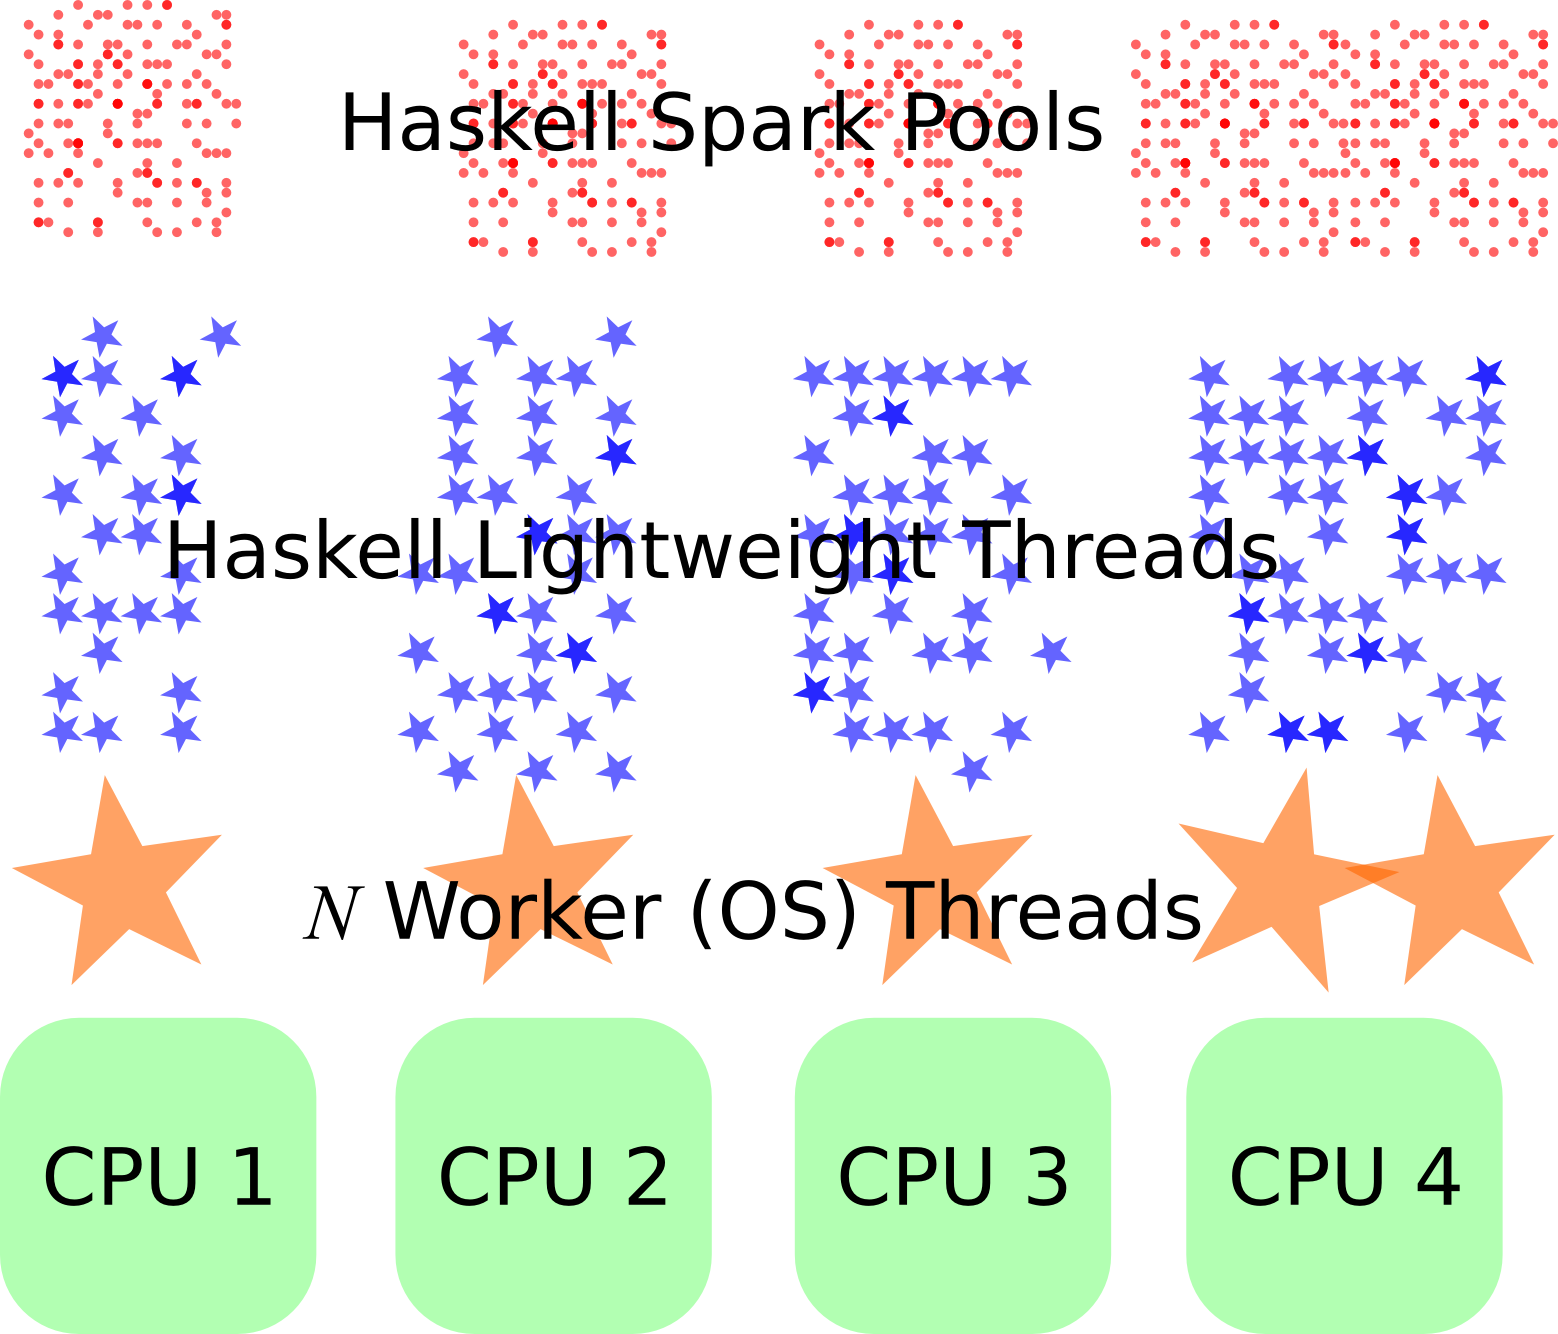
\includegraphics[height=.8\textheight]{sparks}
    \caption{Don Stewart (\href{https://stackoverflow.com/questions/958449/what-is-a-spark-in-haskell}{$\rightarrow$ Stackoverflow-Link})}
\end{figure}
\end{frame}

\begin{frame}
\frametitle{Manuelle Parallelisierung}
    \begin{itemize}
    \item {\color{blue}\texttt{rpar x}} generiert einen Spark für ihr Argument
    \item {\color{blue}\texttt{rseq x y}} sorgt für die Auswertung von \texttt{x} bevor sie \texttt{y} zurückgibt
    \item[$\rightarrow$] {\color{blue}\texttt{y rseq x $\cdot$ y}}
    \end{itemize}
\end{frame}

\begin{frame}
\frametitle{Manuelle Parallelisierung}
    \begin{itemize}
    \item Par Monade
    \end{itemize}
\end{frame}

\subsection{\C++}

\begin{frame}
\frametitle{Manuelle Parallelisierung}
    \onslide<2->{
        \textbf{POSIX-Threads (PThreads)}
        \begin{itemize}
            \item Implementierung des Threadmodells für POSIX-Systeme
            \item \dots
        \end{itemize}
    }

    \vfill

    \onslide<3->{
        \textbf{std::threads}
        \begin{itemize}
            \item Moderene Alternative in Form einer \C++ Standardbibliothek
            \item \dots
        \end{itemize}
    }
\end{frame}

\begin{frame}
\frametitle{Parallele APIs}
    \onslide<2->{
        \textbf{Open Multiprocessing (OpenMP)}
        \begin{itemize}
            \item \dots
        \end{itemize}
    }

    \vfill

    \onslide<3->{
        \textbf{Intel Threading Building Blocks (TBB)}
        \begin{itemize}
            \item \dots
        \end{itemize}
    }
\end{frame}

\begin{frame}
\frametitle{Parallele Standardbibliotheken}
    \begin{itemize}
        \item Offensichtliche Parallelität in Map und Reduce
        \item Eigener Namespace \texttt{std::\_\_parallel}
    \end{itemize}
\end{frame}

%------------------------------------------------
\section{Messergebnisse}

\begin{frame}
\setcounter{subsection}{1}
\tableofcontents[currentsection]
\end{frame}
%------------------------------------------------

\begin{frame}
\frametitle{Quellen}
\printbibliography
\end{frame}

% \begin{thebibliography}{99}
% \bibitem[Flynn 1966]{flynn1966very} Michael J Flynn (1966)
% \newblock Very high-speed computing systems
% \newblock \emph{Proceedings of the IEEE} 54.12, S. 1901--1909
% \bibitem[Dean and Ghemawat 2004]{dean2004} Jeffrey Dean and Sanjay Ghemawat 2004
% \newblock MapReduce: Simplified Data Processing on Large Clusters
% \newblock \emph{6th Symposium on Operating System Design and Implementation, 2004}
% \end{thebibliography}


\begin{frame}
\centering
\Huge{Vielen Dank für Eure Aufmerksamkeit}
\end{frame}

%------------------------------------------------

\end{document} 
